\documentclass[12pt]{article}
\usepackage[margin=0.3in,top=0.25in,bottom=0.4in]{geometry}
\makeatletter
\renewcommand{\@maketitle}{\newpage\null\vskip -3.5em\begin{center}{\LARGE \@title \par}\end{center}\par\vskip 0.2em}
\makeatother
\usepackage{amsmath,amssymb}
\usepackage{graphicx}
\usepackage{booktabs}
\usepackage{tikz}
\usetikzlibrary{arrows.meta}
\usepackage{hyperref}
\setlength{\parskip}{0.6em}
\setlength{\parindent}{0pt}

\title{Why two ways of counting photons give different answers\\
\large A simple explanation of the photon flux}
\author{}
\date{}

\begin{document}
\maketitle

\section*{1. The setting}

Two lead nuclei fly past each other at almost the speed of light, without touching. Each one
carries a strong electric charge, and a fast-moving charge is surrounded by a \textbf{cloud of
photons} (particles of light). One nucleus, the \emph{emitter}, sends a photon to the other one,
the \emph{target}, and the photon hits one of the target's protons or neutrons (nucleons). That
collision is what makes our charm quarks.

To predict how often this happens we need to know \textbf{how many photons reach the target}.
This number is called the \emph{photon flux}.

\section*{2. The photon cloud gets thinner with distance}

The cloud is dense close to the emitter and thin far away, like the light around a lamp. How
quickly it thins out depends on the photon's energy:
\begin{itemize}
\item \textbf{Low-energy photons} form a \emph{huge} cloud. It reaches thousands of times
  farther than the size of a nucleus, and thins out slowly.
\item \textbf{High-energy photons} form a \emph{tiny} cloud, smaller than a nucleus. It thins out
  extremely fast: a few steps away from the emitter there are almost none left.
\end{itemize}

\section*{3. Two ways of counting}

The target is not a point: it is a ball of 208 nucleons, about 13 fm across
(1~fm $=10^{-15}$~m). The photon can hit any of them.

\begin{center}
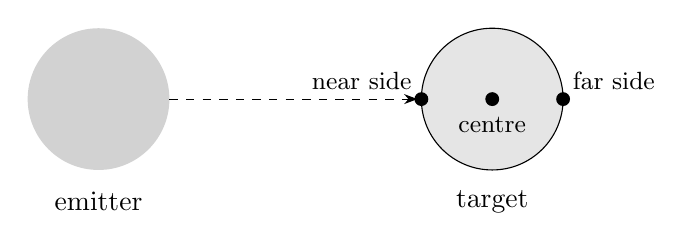
\begin{tikzpicture}[>=Stealth, scale=1.0]
  \fill[gray!35] (0,0) circle (0.9);
  \node at (0,-1.3) {emitter};
  \fill[gray!20] (5,0) circle (0.9);
  \draw (5,0) circle (0.9);
  \node at (5,-1.3) {target};
  \fill (4.1,0) circle (2.5pt);
  \node[above left] at (4.1,0) {\small near side};
  \fill (5,0) circle (2.5pt);
  \node[below] at (5,-0.1) {\small centre};
  \fill (5.9,0) circle (2.5pt);
  \node[above right] at (5.9,0) {\small far side};
  \draw[->, dashed] (0.9,-0.0) -- (4.05,-0.0);
\end{tikzpicture}
\end{center}

\begin{itemize}
\item \textbf{Method 1 (``centre''):} count the photons at the \emph{centre} of the target and
  pretend every nucleon sees that number. This is what Guzey \textit{et al.}\ (arXiv:2606.05469)
  do.
\item \textbf{Method 2 (``average''):} count the photons at the position of \emph{each}
  nucleon, and take the average over all of them. This is what our code does by default
  (the ``EFF'' flux of Eskola \textit{et al.}, arXiv:2404.09731).
\end{itemize}

The two methods should agree if the number of photons is about the same all over the target.
They disagree if it changes a lot from one side of the target to the other.

\section*{4. An everyday example}

Imagine standing in front of a heater.
\begin{itemize}
\item If the heater is \textbf{far away}, your front and your back feel almost the same warmth.
  Measuring the temperature at your belly button (``centre'') or averaging over your whole body
  (``average'') gives the same answer.
\item If the heater is \textbf{very close} and its heat drops very quickly with distance, your
  front gets hot while your back stays cold. Now the average is much larger than the value at
  your belly button, because the hot front side counts a lot and the cold back side cannot be
  colder than ``nothing''.
\end{itemize}

The photon cloud works the same way. For \textbf{low-energy} photons the cloud is huge compared
to the target, so the near side and the far side see almost the same number of photons: the two
methods agree. For \textbf{high-energy} photons the cloud is smaller than the target, so the near
side sees enormously more photons than the centre: the average is much larger.

Why is the target ``very close'' for high-energy photons? Their cloud is so small that they only
reach the target when the two nuclei pass each other as closely as possible, almost touching.
In those fly-bys the near side of the target is only about half as far from the emitter as its
centre. When the nuclei pass farther apart, high-energy photons practically never arrive, so
those fly-bys do not count.

\section*{5. How big is the difference?}

The photon energy is measured by $z_\gamma$, the fraction of the beam energy the photon carries.
Small $z_\gamma$ means low energy, large $z_\gamma$ means high energy.

\begin{center}
\begin{tabular}{ccc}
\toprule
$z_\gamma$ & size of the photon cloud & ``average'' / ``centre'' \\
\midrule
$10^{-4}$ & 2100 fm (huge)      & 1.01 \\
$10^{-3}$ & 210 fm              & 1.02 \\
$10^{-2}$ & 21 fm               & 1.11 \\
$0.03$    & 7 fm (target size)  & 1.7 \\
$0.1$     & 2 fm (tiny)         & 30 \\
\bottomrule
\end{tabular}
\end{center}

So: \textbf{for most photons the two methods agree within a few per cent.} Only for the
highest-energy photons does the average become much bigger, and those photons are rare.
Figure~\ref{fig:flux} shows the same thing: the curves agree on the left and split apart on the
right.

\begin{figure}[h]
\centering
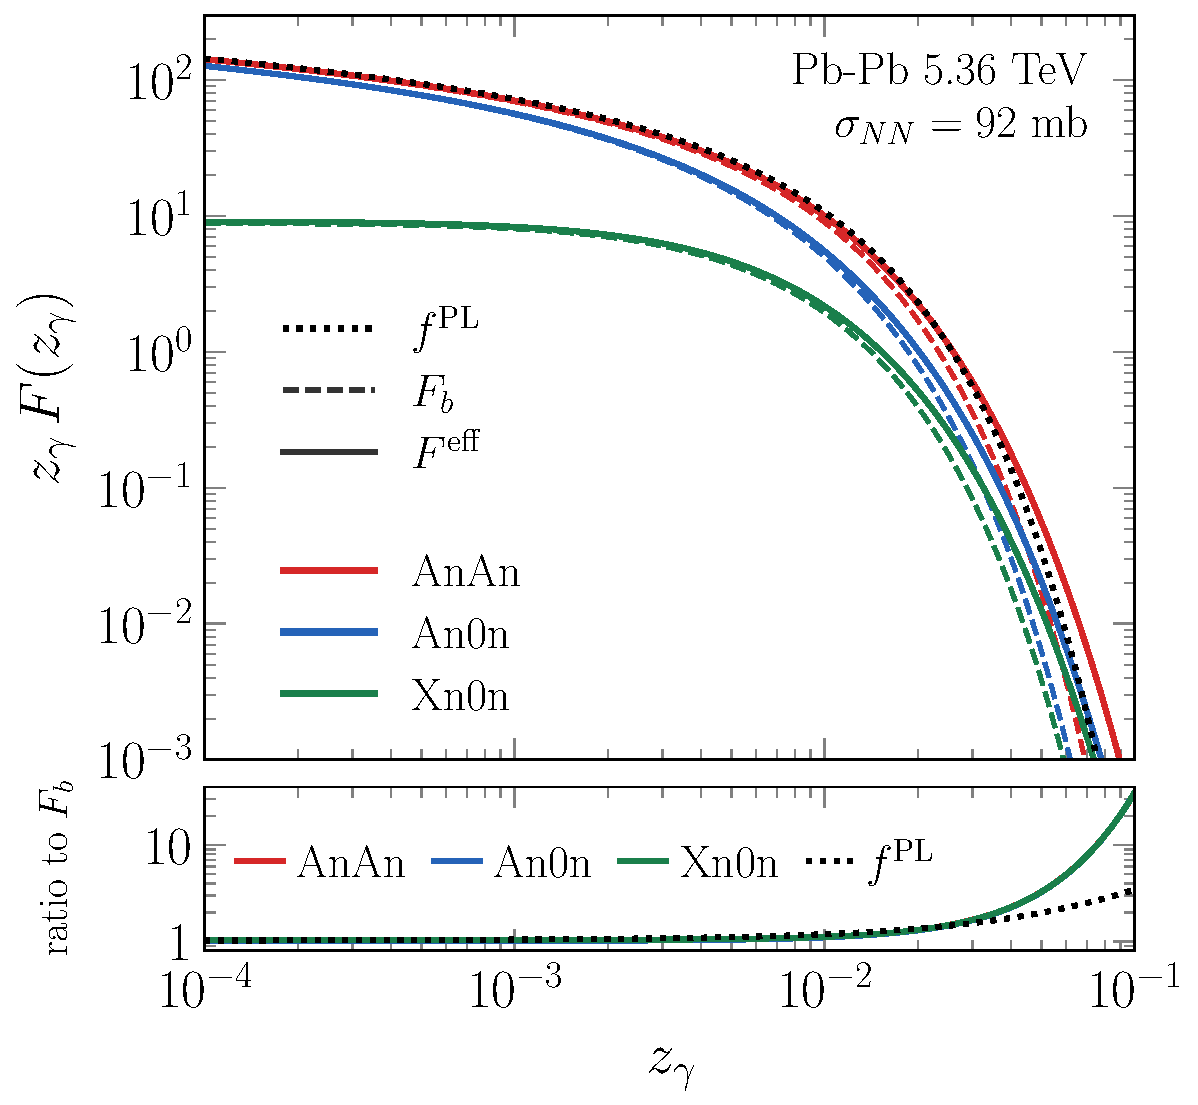
\includegraphics[width=0.6\textwidth]{../plots/flux_eff_vs_ws.pdf}
\caption{Number of photons as a function of the photon energy $z_\gamma$. Dashed: method 1
(centre). Solid: method 2 (average). Dotted: an even simpler version that treats the emitter as a
point. The colours are different neutron selections. The lower panel shows how many times larger each one is
than method 1.}
\label{fig:flux}
\end{figure}

\section*{Where do these numbers come from?}

They come from the formula for how the photon cloud thins out with distance. Figure~\ref{fig:dist}
shows it for one fly-by, with the near side, centre and far side of the target marked. Each curve
is divided by its value at the centre, so all of them pass through 1 there.

\begin{figure}[h]
\centering
\includegraphics[width=0.6\textwidth]{../plots/flux_vs_distance.pdf}
\caption{How many photons there are at each distance from the emitter, compared with the centre
of the target. Low-energy photons (blue, $z_\gamma=10^{-3}$): almost the same everywhere on the
target. High-energy photons (red, $z_\gamma=0.1$): about 1000 times more at the near side, about
1000 times fewer at the far side.}
\label{fig:dist}
\end{figure}

For high-energy photons, moving to the near side \textbf{multiplies} the number of photons by
about 500, and moving the same distance to the far side \textbf{divides} it by about 500. These
are equal factors, but very unequal amounts. Say the centre has 1 photon:
\begin{itemize}
\item near side: $1\times500 = 500$ photons, a gain of 499;
\item far side: $1\div500 = 0.002$ photons, a loss of only 0.998, because you cannot lose more
  than the 1 photon you had.
\end{itemize}
The average of the two sides is about 250, much more than the 1 photon at the centre.

For low-energy photons the factor is only about 1.06: $1\times1.06=1.06$ and $1\div1.06=0.94$.
The gain (0.06) and the loss (0.06) are almost equal, so the average stays at 1.

The rule is simple: \textbf{if the number of photons changes by a large factor across the
target, the average is much bigger than the centre value; if it hardly changes, they are the
same.}

\section*{6. Does it matter for our results?}

Producing a heavier or more forward charm quark needs a more energetic photon. So:
\begin{itemize}
\item at low transverse momentum and central rapidity, our cross sections are only
  \textbf{1--4\%} higher than with method 1;
\item at high transverse momentum and forward rapidity they are higher by about \textbf{17\%}
  ($p_\perp=10$~GeV, $y=2$) and up to \textbf{a factor 2} ($p_\perp=10$~GeV, $y=3$).
\end{itemize}

\section*{7. Which method is right?}

Method 2 is the more realistic one: the photon really does hit a nucleon somewhere inside the
target, not exactly at its centre. Method 1 is a simplification that works well for low-energy
photons, which are the vast majority. Both use the same physics otherwise (same nucleus, same
probability of the nuclei not colliding, same neutron selection). If we want to reproduce the
numbers of Guzey \textit{et al.}\ exactly, we can switch our code to method 1 with
\texttt{FLUX\_MODEL=WS}.

\section*{In one sentence}

High-energy photons stay very close to the nucleus that emits them, so the side of the target
facing the emitter receives far more of them than its centre; averaging over the whole target
captures this, while counting only at the centre misses it.

\end{document}
